%-------------------------
% Resume in Latex
% Author : Puneet Gautam, puneet.gautam0206@gmail.com, punitrajgautam@uiit.ac.in
% License : MIT
%MIT License

%Copyright (c) 2023 Puneet Gautam

%Permission is hereby granted, free of charge, to any person obtaining a copy
%of this software and associated documentation files (the "Software"), to deal
%in the Software without restriction, including without limitation the rights
%to use, copy, modify, merge, publish, distribute, sublicense, and/or sell
%copies of the Software, and to permit persons to whom the Software is
%furnished to do so, subject to the following conditions:

%The above copyright notice and this permission notice shall be included in all
%copies or substantial portions of the Software.

%THE SOFTWARE IS PROVIDED "AS IS", WITHOUT WARRANTY OF ANY KIND, EXPRESS OR
%IMPLIED, INCLUDING BUT NOT LIMITED TO THE WARRANTIES OF MERCHANTABILITY,
%FITNESS FOR A PARTICULAR PURPOSE AND NONINFRINGEMENT. IN NO EVENT SHALL THE
%AUTHORS OR COPYRIGHT HOLDERS BE LIABLE FOR ANY CLAIM, DAMAGES OR OTHER
%LIABILITY, WHETHER IN AN ACTION OF CONTRACT, TORT OR OTHERWISE, ARISING FROM,
%OUT OF OR IN CONNECTION WITH THE SOFTWARE OR THE USE OR OTHER DEALINGS IN THE
%SOFTWARE.
%------------------------

%---- Required Packages and Functions ----

\documentclass[a4paper,11pt]{article}
\usepackage{latexsym}
\usepackage{xcolor}
\usepackage{float}
\usepackage{ragged2e}
\usepackage[empty]{fullpage}
\usepackage{wrapfig}
\usepackage{lipsum}
\usepackage{tabularx}
\usepackage{titlesec}
\usepackage{geometry}
\usepackage{tikz}
\usepackage{marvosym}
\usepackage{verbatim}
\usepackage{enumitem}
\usepackage[hidelinks]{hyperref}
\usepackage{fancyhdr}
\usepackage{multicol}
\usepackage{graphicx}
\usepackage{cfr-lm}
\usepackage[T1]{fontenc}
\usepackage[%
backend=biber
,bibstyle=apa
,citestyle=numeric-comp
,sorting=none
,sortcites=true
,block=none
]{biblatex}

\makeatletter
\RequireBibliographyStyle{numeric}
\makeatother
\addbibresource{references.bib}
\setlength{\multicolsep}{0pt} 
\pagestyle{fancy}
\fancyhf{} % clear all header and footer fields
\fancyfoot{}
\renewcommand{\headrulewidth}{0pt}
\renewcommand{\footrulewidth}{0pt}
\geometry{left=0.6cm, top=0.5cm, right=0.6cm, bottom=0.5cm}
% Adjust margins
%\addtolength{\oddsidemargin}{-0.5in}
%\addtolength{\evensidemargin}{-0.5in}
%\addtolength{\textwidth}{1in}
\usepackage[most]{tcolorbox}
\tcbset{
	frame code={}
	center title,
	left=0pt,
	right=0pt,
	top=0pt,
	bottom=0pt,
	colback=gray!20,
	colframe=white,
	width=\dimexpr\textwidth\relax,
	enlarge left by=-2mm,
	boxsep=4pt,
	arc=0pt,outer arc=0pt,
}

\urlstyle{same}

\raggedright
\setlength{\tabcolsep}{0in}

% Sections formatting
\titleformat{\section}{
  \vspace{-4pt}\scshape\raggedright\large
}{}{0em}{}[\color{black}\titlerule \vspace{-7pt}]

%-------------------------
% Custom commands
\newcommand{\resumeItem}[2]{
  \item{
    \textbf{#1}{:\hspace{0.5mm}#2 \vspace{-0.5mm}}
  }
}

\newcommand{\resumePOR}[3]{
\vspace{0.5mm}\item
    \begin{tabular*}{0.97\textwidth}[t]{l@{\extracolsep{\fill}}r}
        \textbf{#1},\hspace{0.3mm}#2 & \textit{\small{#3}} 
    \end{tabular*}
    \vspace{-2mm}
}

\newcommand{\resumeSubheading}[4]{
\vspace{0.5mm}\item
    \begin{tabular*}{0.98\textwidth}[t]{l@{\extracolsep{\fill}}r}
        \textbf{#1} & \textit{\footnotesize{#4}} \\
        \textit{\footnotesize{#3}} &  \footnotesize{#2}\\
    \end{tabular*}
    \vspace{-2.4mm}
}

\newcommand{\resumeProject}[4]{
\vspace{0.5mm}\item
    \begin{tabular*}{0.98\textwidth}[t]{l@{\extracolsep{\fill}}r}
        \textbf{#1} & \textit{\footnotesize{#3}} \\
        \footnotesize{\textit{#2}} & \footnotesize{#4}
    \end{tabular*}
    \vspace{-2.4mm}
}

\newcommand{\resumePubs}[6]{
\vspace{0.5mm}\item
    \begin{tabular*}{0.98\textwidth}[t]{l@{\extracolsep{\fill}}r}
        \textbf{#1} & \textit{\footnotesize{#3}} \\
        \footnotesize{#2} & \footnotesize{#4} \\
        \footnotesize{\textit{#5}} & \footnotesize{#6}
    \end{tabular*}
    \vspace{-2.4mm}
}

\newcommand{\resumeSubItem}[2]{\resumeItem{#1}{#2}\vspace{-4pt}}

% \renewcommand{\labelitemii}{$\circ$}
\renewcommand{\labelitemi}{$\vcenter{\hbox{\tiny$\bullet$}}$}

\newcommand{\resumeSubHeadingListStart}{\begin{itemize}[leftmargin=*,labelsep=0mm]}
\newcommand{\resumeHeadingSkillStart}{\begin{itemize}[leftmargin=*,itemsep=1.7mm, rightmargin=2ex]}
\newcommand{\resumeItemListStart}{\begin{justify}\begin{itemize}[leftmargin=3ex, rightmargin=2ex, noitemsep,labelsep=1.2mm,itemsep=0mm]\small}

\newcommand{\resumeSubHeadingListEnd}{\end{itemize}\vspace{2mm}}
\newcommand{\resumeHeadingSkillEnd}{\end{itemize}\vspace{-2mm}}
\newcommand{\resumeItemListEnd}{\end{itemize}\end{justify}\vspace{-2mm}}
\newcommand{\cvsection}[1]{%
\vspace{2mm}
\begin{tcolorbox}
    \textbf{\large #1}
\end{tcolorbox}
    \vspace{-4mm}
}

\newcolumntype{L}{>{\raggedright\arraybackslash}X}%
\newcolumntype{R}{>{\raggedleft\arraybackslash}X}%
\newcolumntype{C}{>{\centering\arraybackslash}X}%
%---- End of Packages and Functions ------

%-------------------------------------------
%%%%%%  CV STARTS HERE  %%%%%%%%%%%
%%%%%% DEFINE ELEMENTS HERE %%%%%%%
\newcommand{\name}{Manuel Gomes} % Your Name
\newcommand{\academictitle}{Master of Science} % Your Academic Title
\newcommand{\course}{Mechanical Engineering} % Your Course
\newcommand{\institution}{University of Aveiro, Portugal} % Your Institution
\newcommand{\roll}{Your Roll No} % Your Roll No.
\newcommand{\phone}{} % Your Phone Number
\newcommand{\emaila}{manuelgomes@ua.pt} %Email 1
\newcommand{\emailb}{gomesnelito@gmail.com} %Email 2
\newcommand{\github}{manuelgitgomes} %Github
%\newcommand{\website}{https://www.yourwebsite.com} %Website
\newcommand{\linkedin}{mangomes} %linkedin




\begin{document}
\fontfamily{cmr}\selectfont
%----------HEADING-----------------
\parbox{2.35cm}{%
\begin{tikzpicture}
\clip (0,0)  circle (1cm) ;
\node[anchor=center] at (0,0) {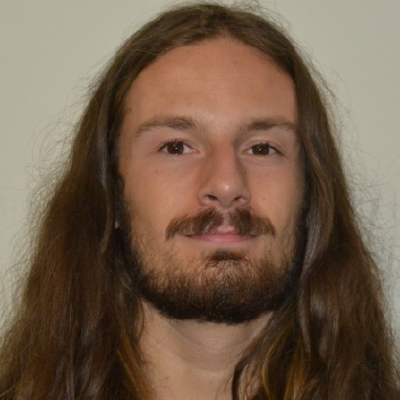
\includegraphics[width=2cm, clip]{figs/manuel.png}}; 
%adjust this coordinate to move image
\end{tikzpicture}
% 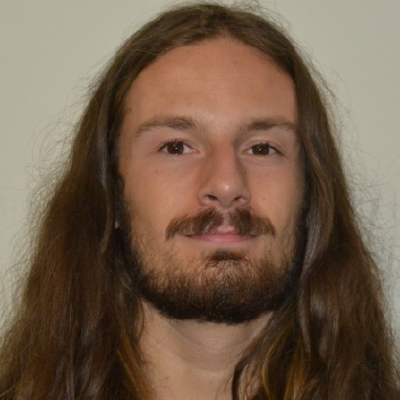
\includegraphics[width=2cm,clip]{figs/manuel.png}

}\parbox{\dimexpr\linewidth-2.8cm\relax}{
\begin{tabularx}{\linewidth}{L r}
  \textbf{\LARGE \name} & \href{mailto:\emaila}{\emaila}\\
  
  \academictitle &  \href{mailto:\emailb}{\emailb}\\
   {in \course} &  \href{https://github.com/\github}{GitHub} \\ %$|$ \href{\website}{Website}\\
  {by the \institution} & \href{https://www.linkedin.com/in/\linkedin/}{LinkedIn}

  % \textbf{\LARGE \name} & +351\phone\\
  
  % \academictitle &  \href{mailto:\emaila}{\emaila}\\
  %  {in \course} &  \href{https://github.com/\github}{GitHub} \\ %$|$ \href{\website}{Website}\\
  % {by the \institution} & \href{https://www.linkedin.com/in/\linkedin/}{LinkedIn}
\end{tabularx}
}

\vspace{-2mm}
%-------------SUMMARY-----------------
\section{\textbf{Summary}}
Ph.D. student with a strong desire to always learn more.
Has previous experience in sensor calibration, mobile robotics, autonomous driving and robotic manipulation.
Has the objective to work as a professor in the future.
%-----------EDUCATION-----------------
\section{\textbf{Education}}
\setlength{\tabcolsep}{6pt} % Default value: 6pt
% \renewcommand{\arraystretch}{1.1} % Default value: 1
\small{\begin{tabularx}
{\dimexpr\textwidth-2mm\relax}{|c|C|c|c|c|}
  \hline
  \textbf{Degree } & \textbf{Institute} & \textbf{University} & \textbf{Evaluation} & \textbf{Year}\\
  \hline
  Ph.D. in Mechanical Engineering & Department of Mechanical Engineering & University of Aveiro & N.A. & 2022 - current \\
  \hline
  \begin{tabular}[c]{@{}c@{}}Integrated M.Sc. (B.Sc. + M.Sc.) \\ in Mechanical Engineering\vspace{-12pt}\end{tabular}  & Department of Mechanical Engineering & University of Aveiro & 17/20 & 2017 - 2022 \\
  \hline
  ERASMUS+ Exchange Program & Faculty of Engineering Technology & University of Twente & N.A. & 2020 \\ 
  \hline
\end{tabularx}}
\vspace{-1mm}

%-----------EXPERIENCE-----------------
\section{\textbf{Experience}}
  \resumeSubHeadingListStart

    \resumeSubheading
      {University of Aveiro}{Aveiro, Portugal}
      {Research Fellow}{March 2022 - current}
      \resumeItemListStart
        \item {Research fellow in the project \href{https://augmanity.pt/}{\emph{AUGMANITY: Augmented Humanity}}}
        \item {Development of a general calibration tool for calibration of various sensors in a collaborative cell}
        \item {Volumetric detection inside a collaborative cell to enhance robot path planning}
      \resumeItemListEnd
    
   \vspace{-1mm}
   \resumeSubheading
     {MAKEIT TECH}{Ílhavo, Portugal}
     {Summer Intern}{June 2021 - October 2021}
     \resumeItemListStart
   \item {Development of a small factor mobile robot to deliver small packages through a complex of offices}
   \item {Projection, design, 3D printing and assembly of mechanical parts}
   \resumeItemListEnd

  %  \vspace{-1mm}
  %  \resumeSubheading
  %    {O2A Autoadesivos}{Albergaria-A-Velha, Portugal}
  %    {Summer Intern}{June 2020 - September 2020}
  %    \resumeItemListStart
  %  \item {Updated factory's inventory, with new products and the respective time taken to produce them}
  %  \resumeItemListEnd
    
    
    % \item {More work done } .....

    
  
      
  \resumeSubHeadingListEnd
\vspace{-6.5mm}
%-----------PROJECTS-----------------
\section{\textbf{Projects}}
\resumeSubHeadingListStart
    
    \resumeProject
      {ATOM Calibration Framework} %Project Name
      {University of Aveiro} %Project Name, Location Name
      {September 2021 - current} %Event Dates
      {\href{https://github.com/lardemua/atom}{\textbf{Github}}} %Website
      \resumeItemListStart
        \item {General calibration framework able to accurately calibrate several sensors with distinct modalities simultaneously}
        \item {Fully integrated into ROS, having visualization and interaction functionalities incorporated}
      \resumeItemListEnd
    
     \vspace{-1mm}
     
    \resumeProject
      {AutoMec AD} %Project Name
      {University of Aveiro} %Project Name, Location Name
      {September 2019 - current} %Event Dates
      {\href{https://github.com/automecua/automec-ad}{\textbf{Github}}} %Website
      \resumeItemListStart
        \item {RC car able to autonomously navigate using a CNN for lane detection and template matching for signal recognition.}
        \item {$4^{th}$ place in the Portuguese Robotic's Festival 2022 Edition}
        \item {Project coordinator since May 2021}
      \resumeItemListEnd
    
\resumeSubHeadingListEnd
\vspace{-7.5mm}

% \section{\textbf{Projects}}
\section{\textbf{Publications \& Talks}}
\resumeSubHeadingListStart
%[1] M. Gomes, M. Oliveira, and V. Santos, “ATOM Calibration Framework: Interaction and Visualization Functionalities,” Sensors, vol. 23, no. 2, Art. no. 2, Jan. 2023, doi: 10.3390/s23020936.

    
    \resumePubs
      {ATOM Calibration Framework: Interaction and Visualization Functionalities} %Project Name
      {\textbf{M. Gomes}, M. Oliveira, V. Santos} %Project Name, Location Name
      {January 2023} %Event Dates
      {\href{https://doi.org/10.3390/s23020936}{\textbf{DOI}: 10.3390/s23020936}} %Website
      {MDPI Sensors, IF (2021): \textbf{3.847}}
      {}
    
    %  \vspace{-2mm}
    \resumePubs
      {ATOM Calibration Framework} %Project Name
      {M. Oliveira, D. Rato, \textbf{M. Gomes}, D. Coelho, E. Pedrosa, N. Lau, V. Santos} %Project Name, Location Name
      {October 2021} %Event Dates
      {\href{https://vimeo.com/showcase/9954564/video/767139832}{\textbf{Video}}} %Website
      {ROSCON 2022, Kyoto}
      {}
     
    \resumePubs
      {A sensor-to-pattern calibration framework for multi-modal industrial collaborative cells} %Project Name
      {D. Rato, M. Oliveira, V. Santos, \textbf{M. Gomes}, A. Sappa} %Project Name, Location Name
      {July 2022} %Event Dates
      {\href{https://doi.org/10.1016/j.jmsy.2022.07.006}{\textbf{DOI}: 10.1016/j.jmsy.2022.07.006}} %Website
      {Journal of Manufacturing Systems, IF (2021): \textbf{9.498}}
      {}

% section{\textbf{Publications \& Talks}}
% \vspace{-0.1mm}
% \resumeSubHeadingListStart
% \resumePOR{M. Gomes, M. Oliveira, and V. Santos, “ATOM Calibration Framework: Interaction and Visualization Functionalities,” Sensors, vol. 23, no. 2, Art. no. 2, Jan. 2023, doi: 10.3390/s23020936.} % Award
%     { About it} % Event
%     {2017} %Event Year
% \vspace{-0.1mm}
% \resumePOR{Achievement 2} % Award
%     {About it} % Event
%     {2021} %Event Year
% \vspace{-0.1mm}
\resumeSubHeadingListEnd
\vspace{-4mm}

\section{\textbf{Technical Skills}}
 \resumeHeadingSkillStart
  \resumeSubItem{Programming Languages} % Category
    {Python, Matlab \& VB.net}
    
    %\vspace{-0.5mm}
    
 \resumeSubItem{Tools and Frameworks} % Category
    {ROS, OpenCV, Jupyter, Visual Studio \& \LaTeX} % Skills
    
    %\vspace{-0.5mm}
    
 \resumeSubItem{Operating Systems} % Category
    {Linux (Ubuntu \& Arch Linux) \& Windows} % Skills
    
    %\vspace{-0.5mm}
    
 
 \resumeHeadingSkillEnd

\vspace{-1.5mm}

\section{\textbf{Key courses taken}}
\resumeHeadingSkillStart
 \resumeSubItem{Computer Science \& Robotics} % Category
    {Autonomous Vehicles, Development \& Analysis of Algorithms, Industrial Systems of Vision and Perception, Intelligent Mobile Robotics, Robotic Systems Programming}
    %\vspace{-0.5mm}
 \resumeSubItem{Electrotechnical and Telecomunications}
 {Automation I, Automation II, Advanced Electrotechnical Instrumentation, Industrial Informatics}
%  \resumeSubItem{Electrical and Electronics} % Category
%     {Advanced Control Systems, Digital Systems, Microprocessors} % Skills
\resumeHeadingSkillEnd

\vspace{-1mm}
%---------------CERTIFICATIONS-------------------
\section{\textbf{Certifications}}
    \resumeItemListStart
        % \item {\href{paste link here}{\textbf{Cambridge Advanced Exam}}} %TODO Add link
        \item {{\textbf{Cambridge Advanced Exam}}} %TODO Add link
        {C2 Level (203) - Cambridge Assessment International Education} 
        % \item {\href{paste link here}{\textbf{ Certificate Name}}}
        % {Certifying Institution Name} %Certifying Authority
        % \item {\href{paste link here}{\textbf{ Certificate Name}}}
        % {Certifying Institution Name} %Certifying Authority
    \resumeItemListEnd
\vspace{-4mm}

%-----------TRAINING-----------------
% \section{\textbf{Vocational Training}}
  % \resumeSubHeadingListStart
  %   \resumeSubheading
  %     {Institution Name}{Location}
  %     {Course Name}{Start Time-EndTime}
  %     \resumeItemListStart
  %       \item {About course, blah blah}
  %       \item {About course, blah blah}
  %     \resumeItemListEnd 
  %   \resumeSubHeadingListEnd


% \section{\textbf{Positions of Responsibility}}
% \vspace{-0.4mm}
% \resumeSubHeadingListStart
%   \resumePOR{Project Coordinator} % Position
%     { AutoMec AD} %Club,Event
%     {May 2021 - Current} %Tenure Period
%   % \resumePOR{Secretary} % Position
%   %   {XYZ Club, UIT Shimla} %Club,Event
%   %   {Apr. 2018 - Apr. 2019} %Tenure Period
% \resumeSubHeadingListEnd
% \vspace{-4mm}


% \section{\textbf{Miscellaneous}}
% \vspace{-0.1mm}
% \resumeSubHeadingListStart
% \resumePOR{Achievement 1} % Award
%     { About it} % Event
%     {2017} %Event Year
% \vspace{-0.1mm}
% \resumePOR{Achievement 2} % Award
%     {About it} % Event
%     {2021} %Event Year
% \vspace{-0.1mm}
% \resumeSubHeadingListEnd
%-------------------------------------------
\vfill
\center{\footnotesize Last updated: \today}

\end{document}
